\documentclass[11pt]{article}
\usepackage[a4paper,margin=25mm]{geometry}
\usepackage{amsmath,amssymb,amsthm,graphicx,booktabs,newunicodechar}
\usepackage[hidelinks]{hyperref}
\newunicodechar{α}{\ensuremath{\alpha}}\newunicodechar{−}{\ensuremath{-}}\newunicodechar{≤}{\ensuremath{\le}}\newunicodechar{≥}{\ensuremath{\ge}}
\newunicodechar{μ}{\ensuremath{\mu}}
\providecommand{\tightlist}{\setlength{\itemsep}{0pt}\setlength{\parskip}{0pt}}
\title{Trial Adaptation with a Background Filter for Fast Reconvergence in Active Control of Impulsive Noise}
\author{Yosuke Sugiura\\Meiji University, Japan}
\date{}
\begin{document}
\maketitle
\begin{abstract}
Adaptive algorithms for active control of impulsive noise prevent divergence by limiting the influence of large samples in the reference and error signals or by using a small step size. These algorithms apply the same update rule to a large error whether it is caused by an impulse or by a sudden change in the primary path. The settings that prevent divergence therefore also slow the reconvergence after the change. This paper proposes a frequency-domain filtered-x algorithm that tests a larger step size on a background filter before the result is used for control. During the test, the foreground filter generates the control signal with its normal step size. When the ratio of the error power to the filtered-reference power rises above a multiple of its running average, the background filter is initialized with the foreground coefficients and adapted with the larger step size. Its coefficients are transferred to the foreground filter only when they give a sufficiently smaller error on the same data. Otherwise, they are discarded, and the control signal is identical to that obtained without the test under the same initial state and input. In simulations with measured room impulse responses and ten noise types, the proposed algorithm reduced the median recovery time after a switch of the noise source by 63\% and 68\% compared with the fastest of nine comparison algorithms. The two values are for new sources close to and far from the original source. For machine gun noise, which consists of intermittent bursts, and for car interior noise with the close source, the trial rarely started, and the comparison algorithm recovered faster. With a fixed primary path, the noise reduction of the two algorithms differed by less than 0.1 dB.
\end{abstract}
\hypertarget{introduction}{%
\section{Introduction}\label{introduction}}

Impulsive noise contains short bursts whose amplitudes are much larger than the background level. Its amplitude distribution has heavier tails than a Gaussian distribution and is often modeled by a symmetric α-stable distribution \cite{shao1993}. In feedforward active noise control (ANC), the filtered-x least-mean-square (FxLMS) algorithm updates the control filter in proportion to the product of the filtered reference signal and the error signal \cite{kuo1996}. An impulsive sample in either signal therefore produces a large update, and such an update can make the control filter diverge.

To prevent this divergence, robust variants of the FxLMS algorithm limit the influence of large samples in the reference and error signals. Sun et al.~\cite{sun2006} ignored the samples that exceeded a threshold, and Akhtar and Mitsuhashi \cite{akhtar2009} replaced them with the threshold values. Wu et al.~\cite{wu2011} minimized the squared logarithm of the error, so that the cost grows slowly for large errors. Other variants are based on M-estimators \cite{wu2013,sun2015} and on fractional lower-order statistics \cite{feng2024}, and Section 2 reviews them. A small step size also reduces the risk of divergence, but it slows the convergence.

These algorithms apply the same update rule to a large error regardless of its cause. A sudden change in the primary path, such as a switch to another noise source, also increases the error, and the error remains elevated while the control filter adapts to the new path. The thresholds, cost functions, and step sizes that prevent divergence under impulses therefore also determine the speed of this reconvergence. In our simulations with measured room impulse responses, we selected the step sizes of nine comparison algorithms to avoid divergence. The fastest of them then needed about 1 s in median to recover after a switch of the noise source (Section 6). This algorithm was our previous frequency-domain algorithm with a coherence-based step size \cite{sugiura2026}.

A larger step size would speed up the reconvergence if it were applied only after a change in the primary path. The ratio of the error power to the filtered-reference power rises after such a change. However, this ratio also rises for other reasons, such as a disturbance at the error microphone, and a larger step size in these cases can degrade the control filter or make it diverge. A rise in the ratio therefore shows only that the primary path may have changed. The proposed algorithm first applies the larger step size to a separate filter and adopts the result only when it reduces the error. We refer to this adaptation as a trial.

The proposed algorithm uses two filters with the same structure. The foreground filter generates the control signal, and the background filter is used only for the trial. When the ratio stays above a multiple of its running average for consecutive blocks, the background filter is initialized with the foreground coefficients and is updated with the larger step size. The foreground filter keeps its normal step size during the trial. The background coefficients are transferred to the foreground filter only after the error computed with them becomes sufficiently smaller than the error computed with the foreground coefficients. Both errors are computed from the measured reference and error signals by using the model of the secondary path. The trial is discarded if this condition is not met within a fixed number of blocks. Because the background filter does not contribute to the control signal, a discarded trial leaves the control signal identical to that obtained without the trial, given the same initial state and input. In contrast, a transfer can also be confirmed when the primary path stays the same. Such a transfer replaces the foreground coefficients and thus affects the control signal. We report how often such transfers occurred.

The trial is useful only if the background filter reduces the error within the trial. For this purpose, the update combines two elements, and we analyze them for finite block lengths. First, the update direction is based on the spectral factor of the filtered-reference power spectrum \cite{elliott2000}, and the step size is divided by the power of each filtered-reference frame relative to its running average. We show that, with the coefficients held fixed, the update caused by an isolated impulse in the reference signal does not depend on the amplitude of the impulse. The algorithm therefore uses impulsive samples without clipping them. Second, whenever the larger step size is used, the error frame is recomputed with the current coefficients, as in the modified FxLMS algorithm \cite{bjarnason1992}. This recomputation applies to start-up, to the trial, and to a fixed number of blocks after a transfer. We derive the form of this update and select its step size below the boundary between decay and growth that we observed in numerical experiments. Our previous algorithm \cite{sugiura2026} had a single filter and used neither element. Ochiai et al.~\cite{ochiai1977} proposed the structure with foreground and background filters for echo cancellation. We apply this structure to the reconvergence of ANC under impulsive noise, and we analyze and evaluate the combined algorithm.

We evaluated the proposed algorithm in closed-loop simulations with room impulse responses measured in one room \cite{meshrir} and with ten noise types (four synthetic signals and six recordings). The recovery time is the time until the short-time error power stays within 3 dB of the level that the same algorithm reaches after the change. Compared with the fastest of the nine comparison algorithms, the proposed algorithm reduced the median recovery time after a switch of the noise source from 0.98 s to 0.36 s for a new source close to the original source and from 1.26 s to 0.40 s for a new source far from it. For machine gun noise, which consists of intermittent bursts, and for car interior noise with the close source, the trial rarely started after the change, and the comparison algorithm recovered faster. Because the reference level of the recovery time depends on the algorithm, we also measured the noise reduction with the coefficients frozen 0.51 s after the switch. Its median was 7.9 dB for the proposed algorithm and 5.0 dB for the comparison algorithm with the close source, and 10.9 dB and 6.8 dB with the far source. With a fixed primary path and no disturbance at the error microphone, the mean noise reduction of the two algorithms differed by less than 0.1 dB over the full 30 s and over the final 10 s.

The remainder of this paper is organized as follows. Section 2 reviews related work, and Section 3 formulates the problem. Section 4 describes the proposed algorithm and its analysis. Section 5 describes the evaluation framework. Section 6 reports the reconvergence after a primary path change, and Section 7 reports the cost of the trial mechanism when the path does not change. Section 8 concludes the paper.

\hypertarget{related-work}{%
\section{Related work}\label{related-work}}

\hypertarget{adaptive-algorithms-for-impulsive-noise}{%
\subsection{Adaptive algorithms for impulsive noise}\label{adaptive-algorithms-for-impulsive-noise}}

The FxLMS algorithm minimizes the mean squared error. For impulsive noise modeled by an α-stable distribution with α \textless{} 2, the second-order moment does not exist \cite{shao1993}. Previous studies therefore modified the update so that large samples have a limited effect on it.

One group of algorithms applies thresholds to the signals. Sun et al.~\cite{sun2006} ignored the samples that exceeded a threshold during adaptation. Akhtar and Mitsuhashi \cite{akhtar2008,akhtar2009} instead replaced such samples in the reference and error signals with the threshold values to obtain faster convergence.

A second group replaces the squared error with a cost function that grows slowly for large errors. Wu et al.~\cite{wu2011} minimized the squared logarithmic transformation of the error. This cost requires no thresholds that depend on the noise statistics. Thanigai et al.~\cite{thanigai2007} used the three-part M-estimator of Hampel to detect and reject impulses in the error signal. Sun et al.~\cite{sun2015} extended this algorithm by passing the reference signal through another Hampel M-estimator with thresholds estimated online. Wu and Qiu \cite{wu2013} reformulated several existing algorithms as M-estimators and proposed an algorithm based on the Fair function. Feng et al.~\cite{feng2024} derived a normalized algorithm from the fractional lower-order covariance and gave its convergence conditions. Cheng et al.~\cite{cheng2023} applied the Gaussian error function to the error and combined it with a normalized variable step size based on a sine function.

In our previous work \cite{sugiura2026}, a frequency-domain FxNLMS algorithm scaled the step size in each frequency bin according to the coherence between the filtered reference and error signals. The scaling factor was limited to a fixed range around the nominal step size.

The algorithms in the two groups bound or compress the contribution of a large error sample to the update. Our previous algorithm keeps a normalized update and changes the step size only within the fixed range. In both cases, one update rule with one set of parameters handles every large error, and these parameters are selected for stability under impulsive noise. The same rule is then applied after a change in the primary path, and it determines the speed of reconvergence (Section 1).

\hypertarget{algorithms-with-two-adaptive-filters}{%
\subsection{Algorithms with two adaptive filters}\label{algorithms-with-two-adaptive-filters}}

Two adaptive filters have been combined to obtain both fast convergence and a small steady-state error. Ferrer et al.~\cite{ferrer2013} applied the convex combination of two filtered-x filters with different step sizes to ANC. Cheng et al.~\cite{cheng2022} combined an FxLMS filter with a filter based on the maximum Versoria criterion for impulsive noise. Yu et al.~\cite{yu2020} combined an FxLMS filter with a filter based on the minimum kernel risk-sensitive loss. In these schemes, a mixing parameter weights the two filters, and both filters contribute to the control signal whenever their weights are nonzero. We include the algorithm of Ferrer et al.~in the evaluation (Section 6).

Ochiai et al.~\cite{ochiai1977} used two filters in a different way. Their echo canceler adapted a background model and used a foreground model to synthesize the echo replica. The model with the smaller residual became the new foreground model. This structure prevented false adaptation during double talk from affecting the echo replica. In echo cancellation, the replica is subtracted electrically, and the residual of each model can be computed directly. In ANC, the control signal reaches the error microphone through the secondary path, and only the error of the foreground filter is measured. The proposed algorithm therefore reconstructs the error of the background filter with the model of the secondary path (Section 2.3).

\hypertarget{frequency-domain-update-and-error-reconstruction}{%
\subsection{Frequency-domain update and error reconstruction}\label{frequency-domain-update-and-error-reconstruction}}

Kuo et al.~\cite{kuo2005} implemented the FxLMS algorithm in blocks to reduce its computational load. Elliott and Rafaely \cite{elliott1997,elliott2000} showed that the bin-normalized frequency-domain LMS algorithm can converge to a biased solution when the filter is constrained to be causal. They applied the spectral factors of the reference power spectrum before and after the causality constraint, and the resulting algorithm converged to the optimal causal filter. For feedforward control, the factorization also includes the minimum-phase part of the plant response. The proposed algorithm follows this construction and factorizes the regularized power spectrum of the filtered reference signal.

Bjarnason \cite{bjarnason1992} proposed the modified FxLMS algorithm. This algorithm estimates the primary noise at the error microphone by subtracting the filtered control signal from the measured error. It then computes the error that the current coefficients would produce. This modification removes the delay of the secondary path from the adaptation loop \cite{yang2018}. The proposed algorithm uses this reconstruction for two purposes. The first is the update with the larger step size during start-up, during a trial, and after a transfer. The second is the comparison between the foreground and background filters.

\hypertarget{problem-formulation}{%
\section{Problem formulation}\label{problem-formulation}}

\hypertarget{signal-model}{%
\subsection{Signal model}\label{signal-model}}

\begin{figure}[t]\centering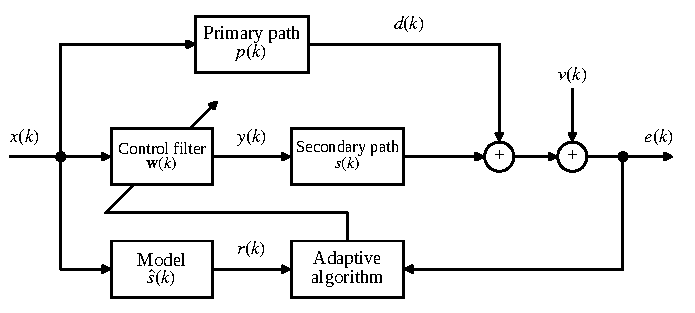
\includegraphics[width=0.8\linewidth]{../fig/fig1.pdf}\caption{Single-channel feedforward ANC system.}\label{fig:system}\end{figure}

Fig. 1 shows the single-channel feedforward ANC system considered in this paper. The reference microphone observes the noise \(x(k)\) at sample \(k\). The noise reaches the error microphone through the primary path \(p(k)\) and produces the primary noise \(d(k) = p(k) * x(k)\), where \(*\) denotes convolution. The control filter has \(M\) coefficients \(\mathbf{w}(k) = [w_0(k), \ldots, w_{M-1}(k)]^{\mathsf T}\) and generates the control signal

\[y(k) = \mathbf{w}^{\mathsf T}(k)\,\mathbf{x}(k), \qquad \mathbf{x}(k) = [x(k), \ldots, x(k-M+1)]^{\mathsf T}.\]

The control signal reaches the error microphone through the secondary path \(s(k)\). The error signal is

\[e(k) = d(k) + s(k) * y(k) + v(k), \tag{1}\]

where \(v(k)\) is a disturbance at the error microphone that is uncorrelated with \(x(k)\). A model \(\hat{s}(k)\) of the secondary path with \(L_s\) coefficients is identified in advance and is fixed during control. The filtered reference signal is \(r(k) = \hat{s}(k) * x(k)\).

\hypertarget{block-frequency-domain-adaptation}{%
\subsection{Block frequency-domain adaptation}\label{block-frequency-domain-adaptation}}

The control signal is computed for every sample in the time domain, so that the control path has no block delay. The coefficients are updated once every \(B\) samples in the frequency domain with the FFT length \(N = 2M\). In block \(n\), \(\mathbf{R}_n = \hat{\mathbf{S}} \odot \mathbf{X}_n\) denotes the spectrum of the filtered reference frame, where \(\mathbf{X}_n\) is the FFT of the latest \(N\) samples of \(x(k)\) and \(\hat{\mathbf{S}}\) is the FFT of \(\hat{s}(k)\). Similarly, \(\mathbf{E}_n\) denotes the FFT of the latest \(M\) samples of \(e(k)\) preceded by \(N - M\) zeros. The frequency-domain FxNLMS algorithm updates the coefficients as

\[\mathbf{w}_{n+1} = \mathbf{w}_n - \mu\, \mathcal{P}_M\, \mathcal{F}^{-1}\!\left\{ \frac{\mathbf{R}_n^{*} \odot \mathbf{E}_n}{\hat{\mathbf{S}}_{rr,n} + \epsilon} \right\}, \tag{2}\]

where \(\mu\) is the step size, \(\hat{\mathbf{S}}_{rr,n}\) is the exponential average of \(|\mathbf{R}_n|^2\), \(\epsilon\) is a regularization constant, \(\odot\) and the division are element-wise, \({}^{*}\) denotes complex conjugation, \(\mathcal{F}^{-1}\) is the inverse FFT, and \(\mathcal{P}_M\) keeps the first \(M\) samples. The projection \(\mathcal{P}_M\) constrains the filter to be causal with \(M\) coefficients. The proposed algorithm replaces the direction and the step size in (2), as described in Section 4.

\hypertarget{impulsive-noise-and-primary-path-change}{%
\subsection{Impulsive noise and primary path change}\label{impulsive-noise-and-primary-path-change}}

The noise \(x(k)\) is impulsive. Its samples occasionally have amplitudes much larger than the background level, and the same impulses appear in \(d(k)\) and, after imperfect cancellation, in \(e(k)\). We place no assumption on the distribution of \(x(k)\) in the algorithm. The evaluation uses a Gaussian signal, a Gaussian signal with isolated impulses, symmetric α-stable signals, and recorded noise (Section 5).

The primary path changes at an unknown sample \(k_c\):

\[p(k) = \begin{cases} p_1(k), & k < k_c, \\ p_2(k), & k \ge k_c. \end{cases} \tag{3}\]

Such a change occurs when the dominant noise source switches to a source at another position. The optimal control filter then changes from the solution for \(p_1\) to the solution for \(p_2\), and the error increases until the control filter reconverges. The secondary path \(s(k)\) and its model \(\hat{s}(k)\) stay the same before and after \(k_c\). A change in the secondary path requires the model \(\hat{s}(k)\) to be identified again, and this paper focuses only on the change in the primary path.

\hypertarget{requirements}{%
\subsection{Requirements}\label{requirements}}

We require the following three properties of the adaptive algorithm under impulsive noise.

\begin{enumerate}
\def\labelenumi{\arabic{enumi}.}
\tightlist
\item
  Reconvergence: after the change in (3), the error power returns to its converged level in a short time. Section 5 defines the recovery time that measures this property.
\item
  Steady state: when the primary path stays the same, the mechanism for fast reconvergence leaves the noise reduction at the level obtained without it.
\item
  Disturbance: when the error increases because of \(v(k)\) in (1) and the primary path stays the same, the mechanism likewise leaves the noise reduction at the level obtained without it.
\end{enumerate}

The first requirement calls for a large update after \(k_c\), and the second and third requirements call for the normal update at all other times. The algorithm observes only \(x(k)\) and \(e(k)\), and \(k_c\) is unknown. Section 4 describes the mechanism, and Section 7 measures the second and third requirements against the same algorithm with the mechanism disabled.

\hypertarget{proposed-algorithm}{%
\section{Proposed algorithm}\label{proposed-algorithm}}

\hypertarget{overview}{%
\subsection{Overview}\label{overview}}

\begin{figure}[t]\centering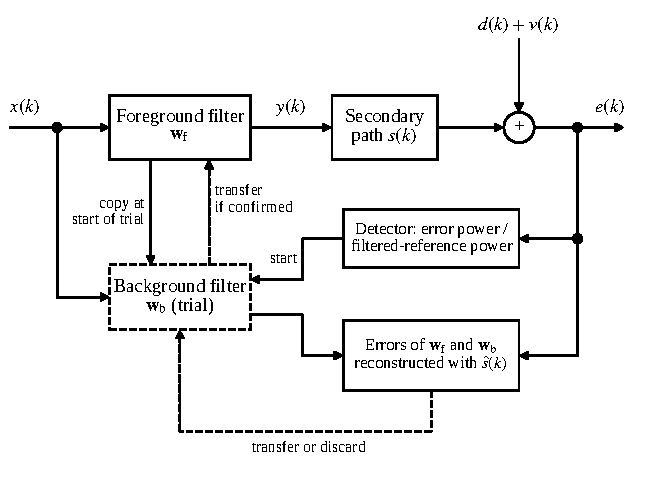
\includegraphics[width=0.8\linewidth]{../fig/fig2.pdf}\caption{Structure of the proposed algorithm. The foreground filter generates the control signal. The background filter is adapted only during a trial, and its coefficients are transferred to the foreground filter or discarded according to the reconstructed errors of the two filters.}\label{fig:structure}\end{figure}

Fig. 2 shows the structure of the proposed algorithm. The foreground filter \(\mathbf{w}_{\mathrm f}\) generates the control signal, and the background filter \(\mathbf{w}_{\mathrm b}\) exists only during a trial. Both filters use the update

\[\mathbf{w}_{n+1} = \mathbf{w}_n - \frac{\sigma_n}{\max(g_n, g_{\min})}\,\frac{2B}{M}\,\boldsymbol{\delta}_n, \tag{4}\]

where \(\boldsymbol{\delta}_n\) is the update direction (Section 4.2), \(g_n\) is the relative power of the filtered-reference frame (Section 4.3), \(g_{\min}\) is its lower bound, and \(\sigma_n\) is the step size. The update has two phases. In the early phase, \(\sigma_n = \sigma_{\mathrm E}\) is large, and the error frame is recomputed with the current coefficients (Section 4.4). In the late phase, \(\sigma_n = \sigma_{\mathrm L}\) is small, and the measured error frame is used (Section 4.5). The foreground filter is in the early phase for the first \(n_{\mathrm E}\) blocks after start-up and after each transfer, and it is in the late phase at all other times. The background filter is always in the early phase. Section 4.6 describes when a trial starts and how it ends. Table 1 lists the parameter values.

\hypertarget{update-direction}{%
\subsection{Update direction}\label{update-direction}}

The direction in (2) normalizes each frequency bin by the power spectrum before the causality constraint. Elliott and Rafaely \cite{elliott2000} showed that this order biases the solution, and they split the normalization into two spectral factors. We follow this construction. Let \(\boldsymbol{\Lambda}_n = \hat{\mathbf{S}}_{rr,n} + \epsilon \bar{P}_n\), where \(\bar{P}_n\) is the mean of \(\hat{\mathbf{S}}_{rr,n}\) over the frequency bins, and let \(\mathbf{F}_n\) be the minimum-phase factor with \(|\mathbf{F}_n|^2 = \boldsymbol{\Lambda}_n\). We compute \(\mathbf{F}_n\) from the real cepstrum of \(\boldsymbol{\Lambda}_n\). The direction is

\[\boldsymbol{\delta}_n = \mathcal{P}_M\, \mathcal{F}^{-1}\!\left\{ \frac{1}{\mathbf{F}_n} \odot \mathcal{F}\, \mathcal{P}_{N/2}\, \mathcal{F}^{-1}\!\left\{ \frac{\mathbf{R}_n^{*} \odot \mathbf{E}_n}{\mathbf{F}_n^{*}} \right\} \right\}, \tag{5}\]

where \(\mathcal{P}_{N/2}\) keeps the first \(N/2\) samples and sets the others to zero. The division by \(\mathbf{F}_n^{*}\) whitens the cross-correlation, \(\mathcal{P}_{N/2}\) removes its noncausal part, and the division by \(\mathbf{F}_n\) maps the result back to the coefficient domain.

\textbf{Proposition 1.} Assume fixed coefficients \(\mathbf{w}\), a stationary \(x(k)\), \(\epsilon = 0\), and \(N \to \infty\). Then

\[\mathrm{E}[\boldsymbol{\delta}_n] = \frac{M_e}{N}\left(\mathbf{w} - [\mathbf{w}_\infty]_M\right),\]

where \(M_e\) is the length of the error window (\(M_e = M\) in this paper), \(\mathbf{w}_\infty\) is the causal Wiener filter of infinite length, and \([\cdot]_M\) keeps its first \(M\) coefficients.

This result follows from the analysis of Elliott and Rafaely \cite{elliott2000}. With fixed coefficients, the expectation of \(\mathbf{R}_n^{*} \odot \mathbf{E}_n\) is proportional to \(S_{rr}W + S_{rd}\), where \(W\) is the frequency response of \(\mathbf{w}\) and \(S_{rd}\) is the cross spectrum of \(r(k)\) and \(d(k)\). The division by \(F^{*}\) gives \(FW + S_{rd}/F^{*}\). The first term is causal and passes \(\mathcal{P}_{N/2}\) unchanged, and the causal part of the second term is \(-FW_\infty\) by the Wiener--Hopf solution. The division by \(F\) then gives \(W - W_\infty\), and \(\mathcal{P}_M\) keeps its first \(M\) coefficients. The factor \(M_e/N\) is the fraction of the frame occupied by the error window. Under these assumptions, the mean update acts as a scalar on the coefficient error, so that all modes of the coefficient error converge at the same rate regardless of the spectrum of \(r(k)\). For the finite length \(N = 2M\) and \(\epsilon = 10^{-2}\) used in this paper, we evaluated the deviation from this scalar action numerically. The eigenvalues of the mean action, normalized by \(M_e/N\), lay between 0.13 and 1.0, and this spread was caused mainly by the regularization.

\hypertarget{step-size-normalized-by-the-relative-frame-power}{%
\subsection{Step size normalized by the relative frame power}\label{step-size-normalized-by-the-relative-frame-power}}

The factor \(\mathbf{F}_n\) follows the exponential average \(\hat{\mathbf{S}}_{rr,n}\), which changes slowly. When a frame contains an impulse, its power is much larger than the average, and \(\boldsymbol{\delta}_n\) grows with the square of the impulse amplitude. We therefore divide the step size by the relative frame power

\[g_n = \frac{\frac{1}{N/2+1}\sum_{f} |R_n(f)|^2}{\bar{P}_n}. \tag{6}\]

\textbf{Proposition 2.} Assume that the coefficients, \(\mathbf{F}_n\), and \(\bar{P}_n\) are fixed, that \(v(k) = 0\), and that \(x(k) = c(k) * [\varsigma(k)\xi(k)]\), where \(c(k)\) is a fixed filter, \(\xi(k)\) is a unit-variance white sequence, and \(\varsigma(k)\) is a deterministic scale. Then each element of \(\boldsymbol{\delta}_n\) is a quadratic form of the samples \(z(k) = \varsigma(k)\xi(k)\) in the frame. If only one sample \(z(k_0)\) in the frame is nonzero, then \(\boldsymbol{\delta}_n = z^2(k_0)\,\mathbf{k}(k_0)\) and \(g_n = z^2(k_0)\,\kappa(k_0)\) with a vector \(\mathbf{k}(k_0)\) and a scalar \(\kappa(k_0)\) that are independent of \(z(k_0)\). The update \(\boldsymbol{\delta}_n / g_n\) is therefore independent of the amplitude of the impulse.

This result follows directly from (5) and (6). With fixed coefficients and \(v(k) = 0\), both \(\mathbf{R}_n\) and \(\mathbf{E}_n\) are linear in the samples \(z(k)\), so that \(\boldsymbol{\delta}_n\) and \(g_n\) are quadratic in them. Proposition 2 concerns an isolated impulse, and it shows that the update caused by such an impulse is bounded without a threshold. The algorithm therefore keeps the impulsive samples in the update. For frames that contain both an impulse and background noise, the ratio \(\boldsymbol{\delta}_n/g_n\) depends on the position of the impulse in the frame, because \(g_n\) measures the power of the whole frame and \(\boldsymbol{\delta}_n\) depends on the part of the response inside the error window. We rely on the simulations for these cases. The lower bound \(g_{\min}\) in (4) limits the step size for frames with low power.

\hypertarget{early-phase-with-recomputed-error-frames}{%
\subsection{Early phase with recomputed error frames}\label{early-phase-with-recomputed-error-frames}}

The error window of block \(n\) contains \(M_e\) samples, and these samples were produced by the coefficients of the last \(M_e/B\) blocks. The measured error frame therefore responds to an update with a delay, and this delay limits the step size. In the early phase, we remove this dependence on past coefficients. As in the modified FxLMS algorithm \cite{bjarnason1992}, the primary noise is estimated as

\[\hat{d}(k) = e(k) - \hat{s}(k) * y(k), \tag{7}\]

and the error frame is recomputed with the coefficients \(\mathbf{w}_n\) to be updated:

\[\tilde{e}_n(k) = \hat{d}(k) + \hat{s}(k) * \left[\mathbf{w}_n^{\mathsf T}\mathbf{x}(k)\right] \tag{8}\]

for the \(M_e\) samples in the window. \(\mathbf{E}_n\) in (5) is then the FFT of \(\tilde{e}_n(k)\).

The recomputed frame changes the form of the update. Assume \(\hat{s} = s\), ideal whitening (\(\boldsymbol{\Lambda}_n = \mathbf{S}_{rr}\), \(N \to \infty\)), and \(g_n = 1\). Let \(\mathbf{v}_n = \mathbf{w}_n - \mathbf{w}_o\) be the coefficient error with respect to a reference filter \(\mathbf{w}_o\), and let \(a = \sigma_{\mathrm E}\,(2B/M)(M_e/N)\). Under these assumptions, (8) gives \(\tilde{\mathbf{e}}_n = \mathbf{X}^r_n \mathbf{v}_n + \mathbf{e}_o\), where \(\mathbf{e}_o\) is the error of \(\mathbf{w}_o\), and the substitution into (5) and (4) gives

\[\mathbf{v}_{n+1} = (\mathbf{I} - a\,\mathbf{G}_n)\,\mathbf{v}_n + \mathbf{b}_n, \qquad \mathbf{G}_n = \mathbf{F}_M^{-1}\,\mathbf{U}_n^{\mathsf T}\mathbf{X}^{r}_n / M_e, \tag{9}\]

where \(\mathbf{U}_n\) and \(\mathbf{X}^r_n\) are the \(M_e \times M\) regression matrices of the whitened filtered reference and of the filtered reference in the window, \(\mathbf{F}_M\) is the \(M \times M\) convolution matrix of the spectral factor, and \(\mathbf{b}_n\) is the contribution of the residual error of \(\mathbf{w}_o\).

Equation (9) contains only the current coefficient error. The matrices \(\mathbf{G}_n\) of consecutive blocks share samples, and we have no closed-form bound on \(a\) for the stability of (9). We therefore examined (9) numerically for white Gaussian input over 64 blocks. The coefficient error decayed for \(a \le 0.55\) and grew for \(a \ge 0.625\), and the decay after 32 blocks was fastest near \(a = 0.375\). Based on this result, we set \(\sigma_{\mathrm E} = 1\) (\(a = 0.25\) for \(g_n = 1\)) and \(g_{\min} = 0.55\) in the early phase, so that \(a/\max(g_n, g_{\min}) \le 0.455\).

\hypertarget{late-phase}{%
\subsection{Late phase}\label{late-phase}}

In the late phase, the measured error frame is used, and the step size is small. We set \(\sigma_{\mathrm L} = 0.0566\) and \(g_{\min} = 0.25\). In preliminary simulations, the noise reduction over the whole run was the same for \(\sigma_{\mathrm L}\) between 0.02 and 0.09.

\hypertarget{trial-with-the-background-filter}{%
\subsection{Trial with the background filter}\label{trial-with-the-background-filter}}

\textbf{Start of a trial.} For each block, the algorithm computes the ratio

\[z_n = \frac{\sum_{k \in \mathcal{W}_M(n)} e^2(k)}{\sum_{k \in \mathcal{W}_{2M}(n)} r^2(k)}, \tag{10}\]

where \(\mathcal{W}_L(n)\) denotes the latest \(L\) samples at block \(n\). The division by the power of \(r(k)\) removes the common scale of the input from the ratio. Let \(\bar{z}_n\) be the exponential average of \(z_n\). A trial starts at block \(n_0\) when \(z_n > \gamma\,\bar{z}_{n-1}\) holds for two consecutive blocks. After a trial starts, the next trial can start only after \(n_{\mathrm G}\) blocks, and \(\bar{z}_n\) is held constant during this interval.

\textbf{Adaptation.} At block \(n_0\), the background filter is set to \(\mathbf{w}_{\mathrm b} = \mathbf{w}_{{\mathrm f}, n_0}\). From block \(n_0 + 1\), it is updated by (4) in the early phase, with the error frame recomputed by (8) with \(\mathbf{w}_{\mathrm b}\). The foreground filter continues its update in its current phase, and the control signal is generated by \(\mathbf{w}_{\mathrm f}\) only.

\textbf{Decision.} For each block \(n \ge n_0 + 2\), the algorithm recomputes the errors of both filters by (8) for the latest \(B\) samples and forms the ratio

\[\rho_n = \frac{\sum_{k \in \mathcal{W}_B(n)} \tilde{e}_{\mathrm b}^2(k)}{\sum_{k \in \mathcal{W}_B(n)} \tilde{e}_{\mathrm f}^2(k)}. \tag{11}\]

Both errors in (11) use the same \(\hat{d}(k)\), so that a common scale of the signals cancels in the ratio. The trial ends by one of the following rules.

\begin{enumerate}
\def\labelenumi{\arabic{enumi}.}
\tightlist
\item
  Discard: if \(\rho_n > \rho_{\mathrm{abort}}\) or \(\rho_n\) is not finite, \(\mathbf{w}_{\mathrm b}\) is discarded.
\item
  Early transfer: if \(n \ge n_0 + n_1\) and \(\rho_n \le \rho_1\), the coefficients are transferred, \(\mathbf{w}_{\mathrm f} \leftarrow \mathbf{w}_{\mathrm b}\).
\item
  Final decision: at \(n = n_0 + n_2\), the coefficients are transferred if \(\rho_n \le \rho_2\), and \(\mathbf{w}_{\mathrm b}\) is discarded otherwise.
\end{enumerate}

After a transfer, the foreground filter continues in the early phase for the remaining \(n_{\mathrm E} - (n - n_0)\) blocks. We use \(\rho_{\mathrm{abort}} = 4\), \((n_1, \rho_1) = (4, 0.25)\), and \((n_2, \rho_2) = (16, 0.5)\).

\textbf{Proposition 3.} Consider two runs of the algorithm with the same initial state and the same input signals. In the first run, the trials are disabled. In the second run, every trial up to block \(n\) is discarded. Then the control signal \(y(k)\) and the foreground coefficients of the two runs are identical up to block \(n\).

\emph{Proof.} The control signal and the update of \(\mathbf{w}_{\mathrm f}\) depend on \(x(k)\), \(e(k)\), and \(\mathbf{w}_{\mathrm f}\). The background filter and the quantities \(z_n\), \(\bar{z}_n\), and \(\rho_n\) are computed from these signals and affect \(\mathbf{w}_{\mathrm f}\) only through a transfer. Without a transfer, the recursions of \(\mathbf{w}_{\mathrm f}\) and \(y(k)\) in the two runs are the same, and their initial states are the same. \(\blacksquare\)

Proposition 3 requires no assumption on the signals or on the accuracy of \(\hat{s}(k)\). It limits the effect of a trial without a path change to the computation during at most \(n_2\) blocks, provided that the trial is discarded. A transfer without a path change is outside the scope of Proposition 3, and it replaces the foreground coefficients. The thresholds in (11) determine how often such a transfer occurs, and we report its frequency in Section 7. Conversely, a path change produces no speed-up if the ratio in (10) stays below its threshold or if the trial is discarded. We report these cases in Section 6.

\hypertarget{computational-cost}{%
\subsection{Computational cost}\label{computational-cost}}

The background filter adds computation only during a trial. Section 7.4 compares the number of multiplications with that of the FxNLMS algorithm.

\hypertarget{evaluation-framework}{%
\section{Evaluation framework}\label{evaluation-framework}}

\hypertarget{acoustic-paths-and-signals}{%
\subsection{Acoustic paths and signals}\label{acoustic-paths-and-signals}}

We evaluated the algorithms in closed-loop simulations at a sampling rate of 16 kHz. The acoustic paths were taken from the MeshRIR dataset \cite{meshrir}, which contains room impulse responses measured in one room from 32 loudspeaker positions to 441 microphone positions. We selected eight combinations of a noise source, a secondary source, and an error microphone. For each combination, the response from the noise source to the microphone was used as the primary path (4096 coefficients), and the response from the secondary source was used as the secondary path (2048 coefficients). The model \(\hat{s}(k)\) was the first 512 coefficients of the secondary path. The reference signal was the source signal itself, so that the reference path and the acoustic feedback were excluded from the evaluation.

The noise signals were of ten types. Four were synthetic: a Gaussian signal, a Gaussian signal with isolated impulses, and symmetric α-stable signals with \(\alpha = 1.45\) and \(\alpha = 1.20\). Six were recordings: machine gun, factory, destroyer engine, and car interior noise from NOISEX-92 \cite{noisex}, valve noise from MIMII \cite{mimii}, and jackhammer noise from SONYC-UST \cite{sonyc}. All signals were high-pass filtered at 100 Hz. Each run lasted 30 s. For each noise type and each condition, we performed 20 runs with different seeds. The seed determined the combination of paths, the random sequence of the synthetic signals, and the starting position in the recordings.

\hypertarget{conditions}{%
\subsection{Conditions}\label{conditions}}

We used five conditions. In the two source-switch conditions, the primary path changed at 15 s to the response from another loudspeaker to the same microphone. The new loudspeaker was the candidate closest to the original noise source in one condition (close source) and the candidate farthest from it in the other (far source). In the no-change condition, the paths were fixed for 30 s. In the two disturbance conditions, the paths were fixed, and white Gaussian noise was added to the error signal for 0.5 s at 10 s and at 20 s. Its power was 0 dB or −10 dB relative to the power of the primary noise. The secondary path and its model were the same in all conditions.

\hypertarget{algorithms}{%
\subsection{Algorithms}\label{algorithms}}

\begin{table*}[tbp]
\centering
\small
\setlength{\tabcolsep}{4pt}
\caption{Settings of the proposed algorithm and selected step sizes of the comparison algorithms}
\label{tab:atsip-1}
\par\medskip
\textbf{Proposed algorithm}\par\smallskip
\resizebox{\ifdim\width>\linewidth\linewidth\else\width\fi}{!}{%
\begin{tabular}{ll}
\toprule
Parameter & Value \\
\midrule
Sampling rate; high-pass cutoff of the input & 16 kHz; 100 Hz \\
Filter length $M$; FFT length $N$; block shift $B$ & 512; 1024; 128 samples (8 ms) \\
Length of $\hat{s}(k)$, $L_s$; error window $M_e$ & 512; 512 samples \\
Weight $\beta$ of $\hat{\mathbf{S}}_{rr,n}$; regularization $\epsilon$ & 0.05; 0.01 \\
Step sizes $\sigma_{\mathrm E}$; $\sigma_{\mathrm L}$ & 1; 0.0566 \\
Lower bound $g_{\min}$ in the early phase; in the late phase & 0.55; 0.25 \\
Length of the early phase $n_{\mathrm E}$ & 32 blocks, counted from the start of the trial after a transfer \\
Windows of $e(k)$ and $r(k)$ in $z_n$ & 512; 1024 samples \\
Weight of the exponential average $\bar{z}_n$; threshold $\gamma$ & 0.05; 4, for two consecutive blocks \\
Interval $n_{\mathrm G}$ before the next trial & 64 blocks, with $\bar{z}_n$ held constant \\
Discard threshold $\rho_{\mathrm{abort}}$ & 4, from block 2 of the trial \\
Transfer rules $(n_1, \rho_1)$; $(n_2, \rho_2)$ & (4, 0.25); (16, 0.5) \\
\bottomrule
\end{tabular}}
\par\medskip
\textbf{Comparison algorithms}\par\smallskip
\resizebox{\ifdim\width>\linewidth\linewidth\else\width\fi}{!}{%
\begin{tabular}{lll}
\toprule
Algorithm & Step size $\mu$ & Other setting \\
\midrule
FxNLMS & 0.01875 & -- \\
Th-FxNLMS & 0.01875 & Clipping at the 1st and 99th percentiles \\
FxlogNLMS & 0.015625 & -- \\
MFxLMM & 0.000125 & -- \\
FxNFLOC & 0.1 & -- \\
EVSS-FxeLMS & 0.003125 & -- \\
FreqFxLMS & 0.0225 & -- \\
CohVSS-FxNLMS & 0.09 & -- \\
C-FXLMS & 0.0375 (fast), 0.009375 (slow) & Normalized component filters \\
MFxNLMS & 0.05 & Regularization 0.001 \\
\bottomrule
\end{tabular}}
\par\medskip
\begin{minipage}{0.98\textwidth}
\footnotesize
The comparison algorithms use one setting for all noise types and conditions (Section 5.3).\par
\end{minipage}
\end{table*}


Table 1 lists the settings. The proposed algorithm used \(M = 512\), \(N = 1024\), and \(B = 128\), and the same parameter values in all runs. We also evaluated the proposed algorithm with the trials disabled, which we refer to as ``no restart.''

The nine comparison algorithms were FxNLMS, the threshold-based algorithm of Akhtar and Mitsuhashi (Th-FxNLMS) \cite{akhtar2008}, FxlogNLMS \cite{wu2011}, MFxLMM \cite{sun2015}, FxNFLOC \cite{feng2024}, EVSS-FxeLMS \cite{cheng2023}, the block frequency-domain FxLMS algorithm (FreqFxLMS) \cite{kuo2005}, our previous algorithm (CohVSS-FxNLMS) \cite{sugiura2026}, and the convex combination algorithm (C-FXLMS) \cite{ferrer2013}. All of them used control filters with 512 coefficients. For each comparison algorithm, we selected the step size from seven values between 1/32 and 2 times the published value. For Th-FxNLMS, we also selected the threshold from four values. For C-FXLMS, we also selected the ratio of the two step sizes from two values and the component filters from the LMS filters of the original paper and their normalized versions. The selection used five seeds that were separate from the 20 seeds of the evaluation. The criterion was the smallest number of diverged runs, followed by the largest noise reduction over 30 s. One setting per algorithm was then used for all noise types and conditions.

\hypertarget{metrics}{%
\subsection{Metrics}\label{metrics}}

The noise reduction is the ratio of the error power to the primary-noise power in decibels. A negative value indicates a reduction. We computed it over the whole run, over the last 10 s, and over the 2 s after each disturbance. For each seed, the values were averaged over the noise types.

The recovery time is defined for each run of the source-switch conditions. The reference level is the short-time error power that the same algorithm reaches after the change. The recovery time is the time from the change until the short-time error power stays within 3 dB of this level for 1 s. A run without recovery by the end is treated as censored, and medians are computed by the Kaplan--Meier method.

The reference level of the recovery time depends on the algorithm. An algorithm that reaches a small noise reduction can therefore have a short recovery time. To compare the algorithms on a common scale, we also measured the noise reduction with frozen coefficients. The coefficients at 0.13 s and 0.51 s after the change were frozen, and the noise reduction of these fixed coefficients was computed over the signal after the change. Its first 256 ms was excluded.

Differences between two algorithms were computed for pairs of runs with the same noise signal and paths. The 95\% confidence interval was obtained by resampling the 20 seeds 2000 times. We call one algorithm better than the other only when this interval excludes zero.

\hypertarget{reconvergence-after-a-primary-path-change}{%
\section{Reconvergence after a primary path change}\label{reconvergence-after-a-primary-path-change}}

\hypertarget{overall-results}{%
\subsection{Overall results}\label{overall-results}}

\begin{table*}[t]
\centering
\small
\setlength{	abcolsep}{4pt}
\caption{Reconvergence after a source switch}
\label{tab:atsip-2}
\par\medskip
\textbf{Median levels}\par\smallskip
\begin{tabular}{llllll}
\toprule
Switch & Metric & Proposed & CohVSS-FxNLMS & C-FXLMS & No restart \\
\midrule
Near & Recovery (s) & 0.360 & 0.976 & 2.536 & 1.048 \\
Near & Noise reduction with frozen coefficients at 0.13 s (dB) & -2.59 & -0.03 & 1.24 & 1.14 \\
Near & Noise reduction with frozen coefficients at 0.51 s (dB) & -7.89 & -5.01 & -1.91 & -3.26 \\
Far & Recovery (s) & 0.400 & 1.256 & 2.784 & 1.128 \\
Far & Noise reduction with frozen coefficients at 0.13 s (dB) & -6.75 & -0.88 & 0.03 & 0.22 \\
Far & Noise reduction with frozen coefficients at 0.51 s (dB) & -10.87 & -6.84 & -3.17 & -4.47 \\
\bottomrule
\end{tabular}
\par\medskip
\textbf{Paired differences}\par\smallskip
\begin{tabular}{lllll}
\toprule
Switch & Metric & Proposed - CohVSS-FxNLMS & Proposed - C-FXLMS & Proposed - No restart \\
\midrule
Near & Recovery (s) & -0.397 [-0.523, -0.282] (172) & -1.409 [-1.688, -1.155] (171) & -0.459 [-0.564, -0.367] (172) \\
Near & Noise reduction with frozen coefficients at 0.13 s (dB) & -3.50 [-4.08, -2.88] (200) & -4.64 [-5.37, -3.91] (200) & -4.58 [-5.26, -3.90] (200) \\
Near & Noise reduction with frozen coefficients at 0.51 s (dB) & -2.70 [-3.17, -2.15] (200) & -5.63 [-6.17, -5.02] (200) & -4.54 [-4.98, -4.08] (200) \\
Far & Recovery (s) & -0.500 [-0.600, -0.384] (172) & -1.765 [-1.997, -1.537] (172) & -0.587 [-0.721, -0.463] (171) \\
Far & Noise reduction with frozen coefficients at 0.13 s (dB) & -4.99 [-5.48, -4.46] (200) & -5.92 [-6.61, -5.29] (200) & -6.25 [-6.92, -5.62] (200) \\
Far & Noise reduction with frozen coefficients at 0.51 s (dB) & -3.81 [-4.29, -3.22] (200) & -6.93 [-7.48, -6.28] (200) & -6.07 [-6.56, -5.50] (200) \\
\bottomrule
\end{tabular}
\par\medskip
\begin{minipage}{0.98\textwidth}
\footnotesize
Recovery uses each method's post-change reference level +3 dB and a Kaplan-Meier median.\par
The noise reduction with frozen coefficients is the residual-to-primary power ratio with the first 256 ms excluded.\par
Differences are paired means with seed-bootstrap 95\% intervals and pair counts in parentheses. Recovery differences use pairs with recovery observed in both runs.\par
\end{minipage}
\end{table*}

\begin{figure}[t]\centering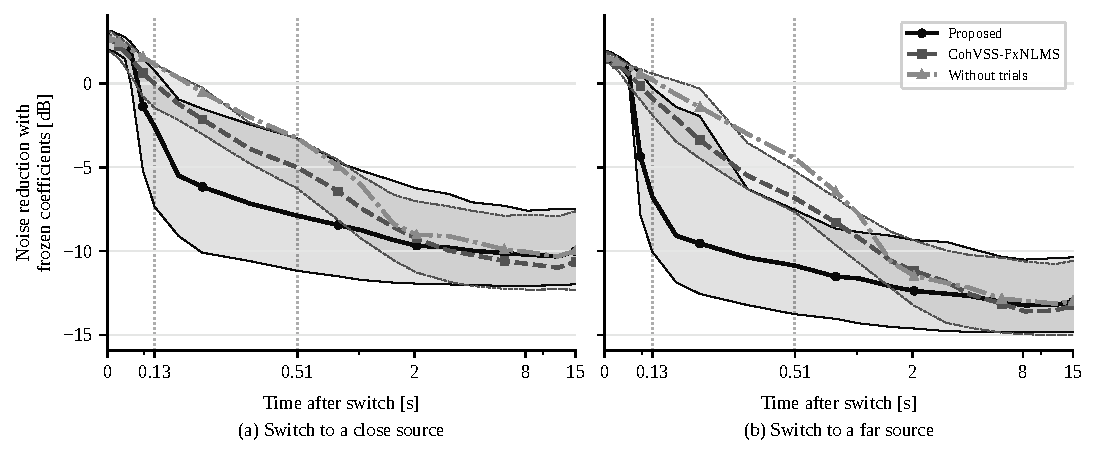
\includegraphics[width=\linewidth]{../fig/fig3.pdf}\caption{Noise reduction with the coefficients frozen at each time after the switch of the noise source (median over 200 runs). The bands show the interquartile range for the proposed algorithm and CohVSS-FxNLMS. The time axis is linear up to 0.55 s and logarithmic thereafter. The vertical dotted lines mark 0.13 s and 0.51 s.}\label{fig:frozen}\end{figure}

No run of the proposed algorithm diverged in the 1000 runs of the five conditions. Table 2 summarizes the two source-switch conditions. The median recovery time of the proposed algorithm was 0.36 s for the close source and 0.40 s for the far source. Among the nine comparison algorithms, CohVSS-FxNLMS had the shortest median recovery times, 0.98 s and 1.26 s. The medians of the other eight algorithms were between 2.3 s and 4.8 s for the close source and between 1.5 s and 5.3 s for the far source. The convex combination did not shorten the recovery: the median of C-FXLMS was 2.54 s and 2.78 s. In C-FXLMS, the mixing parameter stayed above 0.96 before and after the change, so that the fast filter dominated the control signal at all times. The step size of this fast filter had been selected to avoid divergence, and it determined the recovery time.

Fig. 3 shows the noise reduction with frozen coefficients. At 0.13 s after the change, its median was −2.6 dB for the proposed algorithm and −0.0 dB for CohVSS-FxNLMS with the close source, and −6.7 dB and −0.9 dB with the far source. At 0.51 s, the medians were −7.9 dB and −5.0 dB with the close source and −10.9 dB and −6.8 dB with the far source. The paired differences were between −2.7 dB and −5.0 dB, and all four intervals excluded zero (Table 2). After about 2 s, the curves of the two algorithms overlapped.

The proposed algorithm without the trials had median recovery times of 1.05 s and 1.13 s, which are close to those of CohVSS-FxNLMS. The reduction of the recovery time was therefore obtained by the trials.

In the runs with a transfer, the trial started within 2 blocks (median) after the change, and the coefficients were transferred 10 blocks (0.08 s) after the change with the close source and 9 blocks (0.07 s) with the far source.

\hypertarget{results-for-each-noise-type}{%
\subsection{Results for each noise type}\label{results-for-each-noise-type}}

\begin{figure}[t]\centering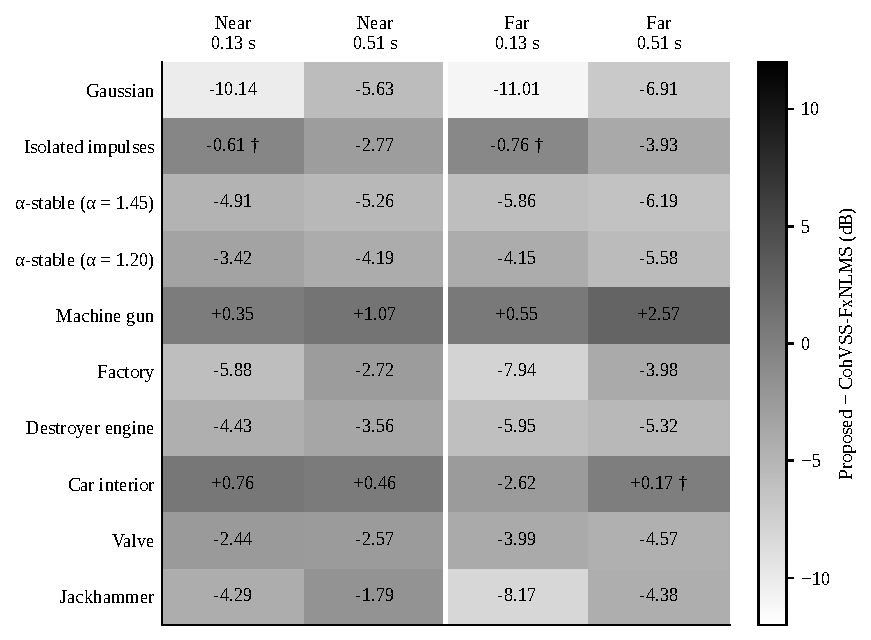
\includegraphics[width=0.75\linewidth]{../fig/fig4.pdf}\caption{Difference in the noise reduction with frozen coefficients between the proposed algorithm and CohVSS-FxNLMS for each noise type (mean of the paired differences over 20 seeds). Negative values indicate a larger noise reduction for the proposed algorithm. A dagger marks a 95\% confidence interval that includes zero.}\label{fig:classes}\end{figure}

Fig. 4 shows the paired difference of the noise reduction with frozen coefficients between the proposed algorithm and CohVSS-FxNLMS for each noise type. Of the 40 comparisons (ten noise types, two conditions, and two times), the proposed algorithm was better in 31, CohVSS-FxNLMS was better in six, and the interval included zero in three. CohVSS-FxNLMS was better for machine gun noise in all four comparisons and for car interior noise with the close source in two comparisons.

These exceptions correspond to the runs in which no trial started after the change. The ratio in (10) did not exceed its threshold in 60 of the 200 runs with the close source and in 20 of the 200 runs with the far source. With the close source, these runs were 20 of the 20 runs for car interior noise, 17 for machine gun noise, eight for valve noise, six for jackhammer noise, five for the isolated impulses, and four for the α-stable signal with \(\alpha = 1.20\). With the far source, they were 11 runs for machine gun noise and nine runs for four other noise types. In such a run, the proposed algorithm operates as the algorithm without the trials, and its control signal is that of this algorithm (Proposition 3).

The two noise types differ from the others in the following respects. Machine gun noise consists of intermittent bursts, and the noise is nearly absent between them. The control filter adapts only during the bursts, and the noise reduction before the change was about 5 dB, compared with 8 dB to 13 dB for the other noise types. The error power relative to the filtered-reference power already varied widely between blocks before the change, so that the change raised the ratio in (10) above its threshold in only five and 12 of the 20 runs. For car interior noise, the switch to the close source raised the error power over the following 2 s by 1.1 dB, which is below the threshold of the detector.

For these noise types, the measured error of the proposed algorithm was not larger than that of CohVSS-FxNLMS. For machine gun noise, the noise reduction of the proposed algorithm over the 2 s after the change was larger by 0.5 dB with the close source ({[}−1.0, −0.1{]} dB) and by 0.3 dB with the far source, where the interval included zero ({[}−0.9, 0.3{]} dB). Over the whole run, it was larger by 0.8 dB and 1.0 dB. For car interior noise with the close source, the difference over the 2 s after the change was −0.1 dB with an interval that included zero, and the noise reduction over the whole run was larger by 0.3 dB. The advantage of CohVSS-FxNLMS for these noise types thus appeared in the recovery time and in the noise reduction with frozen coefficients, and the trial mechanism caused no loss relative to the algorithm without it. The proposed algorithm is intended for noise that is present continuously and contains impulses. Noise that consists only of intermittent bursts requires a detector that operates on the bursts, which we leave for future work.

The recovery time separated the algorithms for five noise types. For the Gaussian signal, the two α-stable signals, factory noise, and destroyer engine noise, the median recovery time of the proposed algorithm was between 0.18 s and 0.35 s, and that of CohVSS-FxNLMS was between 0.74 s and 1.63 s. For valve and jackhammer noise, the recovery times of the two algorithms were the same, although the noise reduction with frozen coefficients was larger for the proposed algorithm by 1.8 dB to 8.2 dB (Fig. 4). The power of these recordings varies over several seconds, and the 3 dB criterion of the recovery time was dominated by this variation. For the isolated impulses, no algorithm met the criterion in any run, and the recovery time could not be evaluated.

\hypertarget{cost-of-the-trial-mechanism}{%
\section{Cost of the trial mechanism}\label{cost-of-the-trial-mechanism}}

This section examines the second and third requirements of Section 3.4 and the contribution of each element. Table 3 summarizes the results.

\hypertarget{no-change-in-the-primary-path}{%
\subsection{No change in the primary path}\label{no-change-in-the-primary-path}}

\begin{table*}[tbp]
\centering
\small
\setlength{\tabcolsep}{6pt}
\caption{Noise reduction with a fixed primary path}
\label{tab:atsip-3}
\par\medskip
\textbf{Levels [dB]}\par\smallskip
\resizebox{\ifdim\width>\linewidth\linewidth\else\width\fi}{!}{%
\begin{tabular}{llllll}
\toprule
Algorithm & \makecell[l]{Whole\\run} & \makecell[l]{Last\\10\,s} & \makecell[l]{2\,s after\\disturbance} & Transfers & \makecell[l]{Identical\\runs} \\
\midrule
\multicolumn{6}{l}{\textit{No change}} \\
Proposed & $-$9.03 & $-$9.11 & -- & 0 & 200/200 \\
CohVSS-FxNLMS & $-$8.98 & $-$9.18 & -- & -- & -- \\
C-FXLMS & $-$8.05 & $-$8.49 & -- & -- & -- \\
MFxNLMS & $-$8.03 & $-$8.34 & -- & -- & -- \\
Without trials & $-$9.03 & $-$9.11 & -- & 0 & -- \\
\multicolumn{6}{l}{\textit{Disturbance (0\,dB)}} \\
Proposed & $-$8.49 & $-$8.15 & $-$5.60 & 13 & 187/200 \\
CohVSS-FxNLMS & $-$8.54 & $-$8.40 & $-$6.22 & -- & -- \\
C-FXLMS & $-$7.67 & $-$7.87 & $-$5.87 & -- & -- \\
MFxNLMS & $-$7.50 & $-$7.45 & $-$5.23 & -- & -- \\
Without trials & $-$8.46 & $-$8.07 & $-$5.59 & 0 & -- \\
\multicolumn{6}{l}{\textit{Disturbance ($-$10\,dB)}} \\
Proposed & $-$8.78 & $-$8.63 & $-$7.45 & 2 & 198/200 \\
CohVSS-FxNLMS & $-$8.77 & $-$8.81 & $-$7.65 & -- & -- \\
C-FXLMS & $-$7.89 & $-$8.23 & $-$7.18 & -- & -- \\
MFxNLMS & $-$7.82 & $-$7.98 & $-$6.89 & -- & -- \\
Without trials & $-$8.78 & $-$8.63 & $-$7.45 & 0 & -- \\
\bottomrule
\end{tabular}}
\par\medskip
\textbf{Paired differences (proposed minus the other algorithm) [dB]}\par\smallskip
\resizebox{\ifdim\width>\linewidth\linewidth\else\width\fi}{!}{%
\begin{tabular}{ll}
\toprule
Other algorithm & Difference [95\% interval] \\
\midrule
\multicolumn{2}{l}{\textit{No change}} \\
CohVSS-FxNLMS & $-$0.053 [$-$0.081, $-$0.025] \\
C-FXLMS & $-$0.983 [$-$1.029, $-$0.935] \\
MFxNLMS & $-$0.999 [$-$1.071, $-$0.928] \\
\multicolumn{2}{l}{\textit{Disturbance (0\,dB)}} \\
CohVSS-FxNLMS & +0.622 [+0.533, +0.715] \\
C-FXLMS & +0.265 [+0.141, +0.395] \\
MFxNLMS & $-$0.371 [$-$0.490, $-$0.244] \\
Without trials & $-$0.011 [$-$0.031, +0.000] \\
\multicolumn{2}{l}{\textit{Disturbance ($-$10\,dB)}} \\
CohVSS-FxNLMS & +0.198 [+0.144, +0.256] \\
C-FXLMS & $-$0.274 [$-$0.358, $-$0.177] \\
MFxNLMS & $-$0.555 [$-$0.659, $-$0.444] \\
Without trials & $-$0.001 [$-$0.002, +0.000] \\
\bottomrule
\end{tabular}}
\par\medskip
\begin{minipage}{0.98\textwidth}
\footnotesize
Differences are taken over the whole run without a change and over the 2\,s after each disturbance otherwise, over 200 runs. Transfers count events in 200 runs. Identical runs are those whose error and control signals equal those of the algorithm without the trials exactly.\par
\end{minipage}
\end{table*}


In the no-change condition, 2494 trials started in the 200 runs. All of them were discarded. The control signal and the error signal of the proposed algorithm were identical to those of the algorithm without the trials in all 200 runs, as stated by Proposition 3. The second requirement was therefore satisfied exactly in this condition.

Compared with CohVSS-FxNLMS, the noise reduction of the proposed algorithm was larger by 0.05 dB over the whole run (95\% confidence interval {[}−0.08, −0.03{]} dB) and smaller by 0.07 dB over the last 10 s ({[}0.04, 0.11{]} dB). Compared with C-FXLMS, it was larger by 0.98 dB over the whole run and by 0.62 dB over the last 10 s. For destroyer engine noise, C-FXLMS had the larger noise reduction, by 0.4 dB over the whole run and by 0.9 dB over the last 10 s.

\hypertarget{disturbance-at-the-error-microphone}{%
\subsection{Disturbance at the error microphone}\label{disturbance-at-the-error-microphone}}

With the 0 dB disturbance, 2641 trials started, and 13 of them ended with a transfer. With the −10 dB disturbance, two of 2520 trials ended with a transfer. No transfer occurred in the no-change condition. The control signal was identical to that of the algorithm without the trials in 187 and 198 of the 200 runs, and every run with a different control signal contained a transfer. In the far-source condition, one transfer occurred in addition to those after the change.

These transfers did not reduce the noise reduction. Over the 2 s after each disturbance, the difference between the proposed algorithm and the algorithm without the trials was −0.01 dB with the 0 dB disturbance and −0.00 dB with the −10 dB disturbance, and both intervals included zero. Over the last 10 s with the 0 dB disturbance, the noise reduction of the proposed algorithm was larger by 0.08 dB ({[}−0.13, −0.04{]} dB). The third requirement was satisfied in this sense.

The comparison algorithms recovered better from the 0 dB disturbance. Over the 2 s after the disturbance, the noise reduction of CohVSS-FxNLMS was larger than that of the proposed algorithm by 0.62 dB, and that of C-FXLMS was larger by 0.27 dB. In C-FXLMS, the mixing parameter fell to 0.04 during the disturbance, so that the slow filter generated the control signal. With the −10 dB disturbance, CohVSS-FxNLMS was better by 0.20 dB, and the proposed algorithm was better than C-FXLMS by 0.27 dB. The proposed algorithm applies its normal update during a disturbance, and the trial does not protect the foreground filter from this update.

\hypertarget{contribution-of-each-element}{%
\subsection{Contribution of each element}\label{contribution-of-each-element}}

We evaluated three variants of the proposed algorithm.

Without the division by \(g_n\), seven to nine of the 200 runs diverged in each condition. The division by the relative frame power was therefore necessary for stability with the early-phase step size.

When the coefficients with the larger step size were used for the control signal as soon as the trial started and were restored if the trial failed, the median recovery times were the same as those of the proposed algorithm (0.36 s and 0.38 s). In the no-change condition, however, the control signal differed from that of the algorithm without the trials in 71 runs. The noise reduction over the whole run was smaller than that of the proposed algorithm by 0.02 dB ({[}−0.03, −0.02{]} dB).

When a trial was started every \(n_2\) blocks without the detector, the median recovery times were 0.30 s and 0.36 s, and no path change was missed by the detector. This variant transferred the coefficients 96 times in the no-change condition and 248 times with the 0 dB disturbance. In the no-change condition, its noise reduction was smaller than that of the proposed algorithm by 0.01 dB. With the 0 dB disturbance, it was larger by 0.50 dB over the 2 s after the disturbance ({[}0.37, 0.64{]} dB), because the transfers replaced the coefficients degraded by the disturbance. The cost of this variant is the computation: a trial is active in every block.

\hypertarget{computational-cost-1}{%
\subsection{Computational cost}\label{computational-cost-1}}

Table 3 lists the number of real multiplications per block of 128 samples, including the sample-by-sample filtering for the control signal. A block in the late phase requires 118,016 multiplications, which is 0.60 times that of the time-domain FxNLMS algorithm with the same filter lengths (196,608). A block with a trial requires 241,920 multiplications (1.23 times). In the eight runs used for this count, a trial was active in 7\% of the blocks, and the average was 126,980 multiplications (0.65 times). The detector thus keeps the average cost below that of the FxNLMS algorithm, and the peak cost exceeds it during a trial.

\hypertarget{conclusion}{%
\section{Conclusion}\label{conclusion}}

This paper proposed a frequency-domain filtered-x algorithm for active control of impulsive noise that tests a larger step size on a background filter and transfers the result to the foreground filter only when it reduces the reconstructed error. We showed that a discarded trial leaves the control signal identical to that obtained without the trial. In simulations with room impulse responses measured in one room and ten noise types, the median recovery time after a switch of the noise source was 0.36 s and 0.40 s, compared with 0.98 s and 1.26 s for the fastest of nine comparison algorithms. With a fixed primary path, the control signal was identical to that of the algorithm without the trials in all runs, and 15 transfers occurred in the 400 runs with a disturbance at the error microphone without reducing the noise reduction.

The proposed algorithm has three limitations. First, the trial did not start after the change in 60 and 20 of the 200 runs of the two source-switch conditions, mainly for machine gun noise, which consists of intermittent bursts, and for car interior noise with a small change in the primary path. In these runs, the proposed algorithm operated as the algorithm without the trials, and the comparison algorithm had the shorter recovery time. Second, after a disturbance at the error microphone, two comparison algorithms had a larger noise reduction by 0.3 dB to 0.6 dB. Third, the evaluation was limited to simulations with paths from one room, a fixed secondary path, and a reference signal without acoustic feedback. Future work includes a detector for noise with intermittent bursts, the evaluation with paths from other rooms, and a real-time implementation.

\bibliographystyle{ieeetr}
\bibliography{refs}
\end{document}
